\documentclass{../cshonours}
\usepackage{subfiles}
\usepackage[table]{xcolor}
\usepackage{url}
\usepackage{graphics}
\usepackage{etoolbox}
\usepackage{bibunits}
\usepackage{amsfonts}
\usepackage{fixltx2e}
\usepackage{tabularx}
\usepackage{accsupp}
\usepackage{pifont}
\usepackage{abbrevs}
\usepackage{acronym}
\usepackage[plain]{fancyref}
\usepackage{threeparttable}
\usepackage{tikz}
\usepackage{hyperref}
\usepackage{xspace}
\usepackage{ccicons}
\usepackage{textcomp}
\usepackage{multicol}
\usepackage{enumerate}
\usepackage{rotating}
\usepackage{tabularx}
\usepackage{calc}
\usepackage{color}
\usepackage[chapter]{minted}
\usepackage{pdflscape}
\usepackage{upquote}
\usepackage{afterpage}
\usepackage{verbatim}
\usepackage{float}
\usepackage{rotfloat}
\usepackage{gensymb}
\usepackage{gnuplot-lua-tikz}
\usepackage{subcaption}
\usepackage{afterpage}

% Avoid PDF inclusion errors
\pdfoptionpdfminorversion=6

% Blank page command
\newcommand\blankpage{%
    \null
    \thispagestyle{empty}%
    \addtocounter{page}{-1}%
    \newpage}

\newcommand{\thetitle}{Towards a Low-Cost, Non-Invasive System for Occupancy Detection using a Thermal Detector Array}
\newcommand{\theauthor}{Ash Tyndall}

\newcommand{\thekeywords}{Energy Saving, Internet of Things, Low-Cost Sensing, Non-Invasive Sensing, Occupancy Sensing, Smart Homes, Thermal Sensing}
\newcommand{\thecategories}{J.7, C.3}

%%% BEGIN LATEX TWEAKS

% Tikz initialize
\usetikzlibrary{shapes, arrows, positioning, fit}
\tikzstyle{dashbox} = [rectangle, dashed, draw=black]
\tikzstyle{box} = [rectangle, draw=black, minimum width=3cm, minimum height=1cm, text centered, text width=3cm]
\tikzstyle{cbox} = [cloud, cloud puffs=15.7, minimum height=1cm, draw]
\tikzstyle{line} = [thin,-,>=stealth]
\tikzstyle{fbox} = [box, dotted, rounded corners=1mm]
\tikzstyle{fcont} = [rectangle, draw=black, minimum width=6cm, minimum height=2.5cm, text centered, text width=6cm]
\tikzstyle{circ} = [circle, draw=black, text centered,  minimum width=2cm, text width=2cm]

% Check marks and cross marks
\newcommand{\cmark}{\hspace{7mm}\BeginAccSupp{ActualText=Y}\checkmark\EndAccSupp{}}
\newcommand{\xmark}{\hspace{7mm}\BeginAccSupp{ActualText=N}\ding{55}\EndAccSupp{}}
\newcommand{\ssup}{\textsuperscript{1}}
\newcommand{\tsup}{\textsuperscript{2}}

% Configure bibliography
\bibliographystyle{acm}
\defaultbibliography{../references/primary}
\defaultbibliographystyle{acm}

% Namelist stuff for proposal
\newcommand{\namelistlabel}[1]{\mbox{#1}\hfil}
\newenvironment{namelist}[1]{%1
\begin{list}{}
    {
        \let\makelabel\namelistlabel
        \settowidth{\labelwidth}{#1}
        \setlength{\leftmargin}{1.1\labelwidth}
    }
  }{%1
\end{list}}

% Additional table options
\newcommand*{\csbox}[1]{\parbox[c]{1.7cm}{\centering #1}}
\newcolumntype{"}{@{\hskip\tabcolsep\vrule width 1pt\hskip\tabcolsep}}

% Acronyms for common stuff
\newcommand{\acrodefn}[3]{%
	\acrodef{#1}[#2]{#3}%
	\expandafter\newcommand\csname#1\endcsname{\ac{#1}\xspace}%
}

\acrodefn{pir}{PIR}{Passive Infrared Sensor}
\acrodefn{iar}{TDA}{Thermal Detector Array}
\acrodefn{lrtda}{lrTDA}{low-resolution Thermal Detector Array}
\acrodefn{mlx}{MLX}{Melexis MLX90620}
\acrodefn{emwa}{EMWA}{Exponential Weighted Moving Average}
\acrodefn{lowpan}{6LoWPAN}{IPv6 over Low power Wireless Personal Area Networks}
\acrodefn{coap}{CoAP}{Constrained Application Protocol}
\acrodefn{iot}{IoT}{Internet of Things}
\acrodefn{rest}{REST}{Representational state transfer}
\acrodefn{roll}{RPL}{IPv6 Routing Protocol for Low-Power and Lossy Networks}
\acrodefn{ws}{WS-*}{Web Services Descriptive Language / Simple Object Access Protocol}
\acrodefn{tarl}{TArL}{the Thermal Array Library}

% Abbreviation commands for common stuff
\newcommand{\cdi}{CO\textsubscript{2}\xspace}
\newcommand{\etal}{et~al.\xspace}
\newcommand{\iic}{$\textrm{I}^2\textrm{C}$\xspace}
\newcommand{\geye}{Grid-EYE\xspace}
\newcommand{\ard}{Arduino\xspace}
\newcommand{\dc}{\degree\textrm{C}\xspace}

% Fancyref support for subsections, source; https://github.com/openlilylib/tutorials/blob/master/aGervasoni/orchestralScores/example-materials/OLLbase.sty
\newcommand*{\fancyrefsubseclabelprefix}{subsec}

\fancyrefaddcaptions{english}{%
  \providecommand*{\frefsubsecname}{subsection}%
  \providecommand*{\Frefsubsecname}{Subsection}%
}

\frefformat{plain}{\fancyrefsubseclabelprefix}{\frefsubsecname\fancyrefdefaultspacing#1}
\Frefformat{plain}{\fancyrefsubseclabelprefix}{\Frefsubsecname\fancyrefdefaultspacing#1}

\frefformat{vario}{\fancyrefsubseclabelprefix}{%
  \frefsubsecname\fancyrefdefaultspacing#1#3%
}
\Frefformat{vario}{\fancyrefsubseclabelprefix}{%
  \Frefsubsecname\fancyrefdefaultspacing#1#3%
}

% Fancyref support for subsubsections, source; https://github.com/openlilylib/tutorials/blob/master/aGervasoni/orchestralScores/example-materials/OLLbase.sty
\newcommand*{\fancyrefsubsubseclabelprefix}{subsubsec}

\fancyrefaddcaptions{english}{%
  \providecommand*{\frefsubsubsecname}{subsection}% the same as for subsection
  \providecommand*{\Frefsubsubsecname}{Subsection}%
}

\frefformat{plain}{\fancyrefsubsubseclabelprefix}{\frefsubsubsecname\fancyrefdefaultspacing#1}
\Frefformat{plain}{\fancyrefsubsubseclabelprefix}{\Frefsubsubsecname\fancyrefdefaultspacing#1}

\frefformat{vario}{\fancyrefsubsubseclabelprefix}{%
  \frefsubsubsecname\fancyrefdefaultspacing#1#3%
}
\Frefformat{vario}{\fancyrefsubsubseclabelprefix}{%
  \Frefsubsubsecname\fancyrefdefaultspacing#1#3%
}

% Fancyref support for listings, source; http://tex.stackexchange.com/questions/70835/how-to-extend-fancyref-for-listings
\newcommand*{\fancyreflstlabelprefix}{lst}

\fancyrefaddcaptions{english}{%
  \providecommand*{\freflstname}{listing}%
  \providecommand*{\Freflstname}{Listing}%
}

\frefformat{plain}{\fancyreflstlabelprefix}{\freflstname\fancyrefdefaultspacing#1}
\Frefformat{plain}{\fancyreflstlabelprefix}{\Freflstname\fancyrefdefaultspacing#1}

\frefformat{vario}{\fancyreflstlabelprefix}{%
  \freflstname\fancyrefdefaultspacing#1#3%
}
\Frefformat{vario}{\fancyreflstlabelprefix}{%
  \Freflstname\fancyrefdefaultspacing#1#3%
}

% Enable subsubsections
\setcounter{secnumdepth}{3} % Enable level 4-5
\setcounter{tocdepth}{3}    % Include level 4-5 in TOC

% Reset acronym definitions in each section and chapter
\preto\section\acresetall
\preto\chapter\acresetall

% Hyperref setup
\hypersetup{pdftitle=\thetitle,pdfauthor=\theauthor,pdfsubject=\thecategories,pdfkeywords=\thekeywords,hidelinks}

% Square table config
\newcolumntype{z}[1] {
  @{{\centering \parbox[c]{\tabcolsep}{\rule{0pt}{#1 + 2\tabcolsep}}}}
  >{\centering\arraybackslash}
  m{#1} }
% 
\renewcommand{\tabularxcolumn}[1]{z{#1}}

% TOC in PDF bookmarks
\makeatletter
\usepackage{etoolbox}
\pretocmd{\tableofcontents}{%
  \if@openright\cleardoublepage\else\clearpage\fi
  \pdfbookmark[0]{\contentsname}{toc}%
}{}{}%
\makeatother

\makeatletter
\usepackage{etoolbox}
\pretocmd{\listoffigures}{%
  \if@openright\cleardoublepage\else\clearpage\fi
  \pdfbookmark[0]{\listfigurename}{lof}%
}{}{}%
\makeatother

\makeatletter
\usepackage{etoolbox}
\pretocmd{\listoftables}{%
  \if@openright\cleardoublepage\else\clearpage\fi
  \pdfbookmark[0]{\listtablename}{lot}%
}{}{}%
\makeatother

% Fix list of listings with minted
\renewcommand{\listoflistings}{%
  \cleardoublepage
  %\addcontentsline{toc}{chapter}{\listoflistingscaption}%
  \listof{listing}{\listoflistingscaption}%
}

% Configure titles
\title{\thetitle}
\author{\theauthor}
\keywords{\thekeywords}
\categories{\thecategories}
%%% END LATEX TWEAKS

\begin{document}
\newcommand{\mainfile}{} % we use the existance of this command to see if we're compiling the whole thesis or just a chapter

\maketitle

% TODO: Mention both ThermoSense and our RMSE.
\begin{abstract}
With the increasing inter-networked and inexpensive nature of embedded sensors and systems, occupancy sensing, the detection of the presence and number of people in a given space, is becoming a cost-effective area of research. Knowing the number of occupants in a space can help reduce energy consumption and greenhouse gas emissions in both small homes and in large office buildings through more efficient climate control. The goal of this project was to develop an occupant sensing system that is low-cost, non-invasive, reliable and energy efficient.

After examining the available sensing options, we concluded that a \lrtda would be the most appropriate sensor for our project, as it has non-invasiveness advantages. The key paper in this area developed the ``ThermoSense'' system using an \lrtda in combination with image subtraction, feature extraction and machine learning classification algorithms. They made occupancy predictions with a Root Mean Squared Error (RMSE) of only 0.35 occupants, at an estimated cost of 170~AUD. However, due to component availability issues, ThermoSense could not be directly replicated in the Australian market.

We designed our own sensing system for 185~AUD using an Arduino, a Raspberry Pi, and a different \lrtda (the MLX90620), which had a narrower, rectangular field of view. The system consumes $\sim$256~mW when active. We also developed \tarl, a software library that implemented ThermoSense's occupant detection algorithm. We then investigated ThermoSense's classification methods, which used numeric Multi-Layer Perceptron, $k$-Nearest Neighbors and Linear Regression algorithms and found our results differed from theirs significantly in both RMSE and correlation, with both being lower. These results suggest that classifiers used are sensitive to the specific sensor's properties.

After further experimentation with our own suite of nominal classification algorithms, we found an approach (K*) that achieved an RMSE of 0.304 and a precision of 82\%, which improves upon ThermoSense's results. We reflected upon our four criteria, and with our choice of sensor, falling component costs, our accuracy results and power consumption statistics, we concluded that our sensing system prototype met our defined criteria.
\end{abstract}

\newpage
\null
\vfill 
\noindent{\fontsize{40pt}{1em}\selectfont \ccbysa}

\null

\noindent\textcopyright\xspace 2014--15 Ashley Ben Tyndall, \url{http://ash.id.au/}

\noindent This document is released under the Creative Commons Attribution-ShareAlike 4.0 International License. A copy of this license can be found at \\ \url{http://creativecommons.org/licenses/by-sa/4.0/}.

\noindent The \LaTeX{} source of this document and supporting files, such as raw data and diagrams, can be found at \url{http://ash.id.au/honours}.

\noindent The following text can be used to satisfy attribution requirements:

\noindent ``This work is based on the honours research project of Ash Tyndall, developed with the help of the School of Computer Science and Software Engineering at The University of Western Australia. A copy of this project can be found at \\ \url{http://ash.id.au/honours}.''
	
\noindent Code and code excerpts included in this document are instead released under the GNU General Public License v3 (\url{http://gnu.org/copyleft/gpl.html}), and can be found in their entirety at the same URL.

\newpage

\begin{acknowledgements}
Writing this dissertation has been my first substantial foray into academic research, and I could not have done it without the assistance and support of so many people.

Firstly, my supervisors Professor Rachel Cardell-Oliver and Professor Adrian Keating have been fundamental to this project's success. Rachel's ability to steer me away from completely redefining the project's parameters at every setback has been of critical importance, as has been her encouragement and computer science advice. Similarly, without Adrian's enviable knowledge of electronics, his skill in constructing prototypes, and his valuable perspective on thermal sensing, this project could not have happened.

Secondly, I wish to acknowledge the generous support of the University, the University Alumni, and the Hackett Foundation through the Hackett Foundation Alumni Honours Scholarship, which I was awarded at the beginning of my project. The financial support this scholarship provided has allowed me to commit more of my time to my research over working, and I can safely say that without it, my research would be of a much poorer quality.

Thirdly, thank you to my friends and family, who have provided support and encouragement throughout this project. I cannot imagine where I would be right now without them. In particular, thank you to Alyssa for your edits, and Magnus and Mark for spending hours with me making revisions.

Additionally, I would like to acknowledge Alex Beltran, Varick L. Erickson and Alberto E. Cerpa, the authors of ThermoSense~\cite{beltran2013thermosense}. Without their groundwork on thermal occupancy sensing, nothing in this dissertation would be possible.

Finally, I would like to acknowledge Linda Salzman Sagan, ``Tompw'' and ``Holek'', the authors of \url{http://commons.wikimedia.org/wiki/File:Human_outline.svg}, which I have adapted for \Fref{fig:exps:3setup}.
\end{acknowledgements}

\tableofcontents
\listoftables
\listoffigures
\listoflistings


\subfile{../introduction/introduction.tex}
\subfile{../litreview/litreview.tex}
\subfile{../design/design.tex}
\subfile{../evaluation/evaluation.tex}
\subfile{../conclusion/conclusion.tex}

\addcontentsline{toc}{chapter}{Bibliography}
\bibliography{../references/primary}

%TC:ignore
\appendix
\chapter{Physical Form}
% TODO: Add scale to photos
To enable the prototype to be easily mounted on the ceiling, the prototype was placed on a flat board with feet that would enable it to be screwed into a pole, and the pole extended to jam the sensor against the ceiling and the floor using the pole (\Fref{fig:pictures:protob1}, \Fref{fig:pictures:protoact}). Due to a wireless module and battery pack being added to the Raspberry Pi, it was feasible for the sensor to operate entirely wirelessly for several hours. However, in most cases it was more convenient to operate using wired power and Ethernet.

\begin{figure}[H]
\centering
\includegraphics[height=0.5\textheight]{../diagrams/prototype-mounted-ceiling.jpg}
\caption{Prototype in action}
\label{fig:pictures:protoact}
\end{figure}

\begin{figure}[H]
\centering
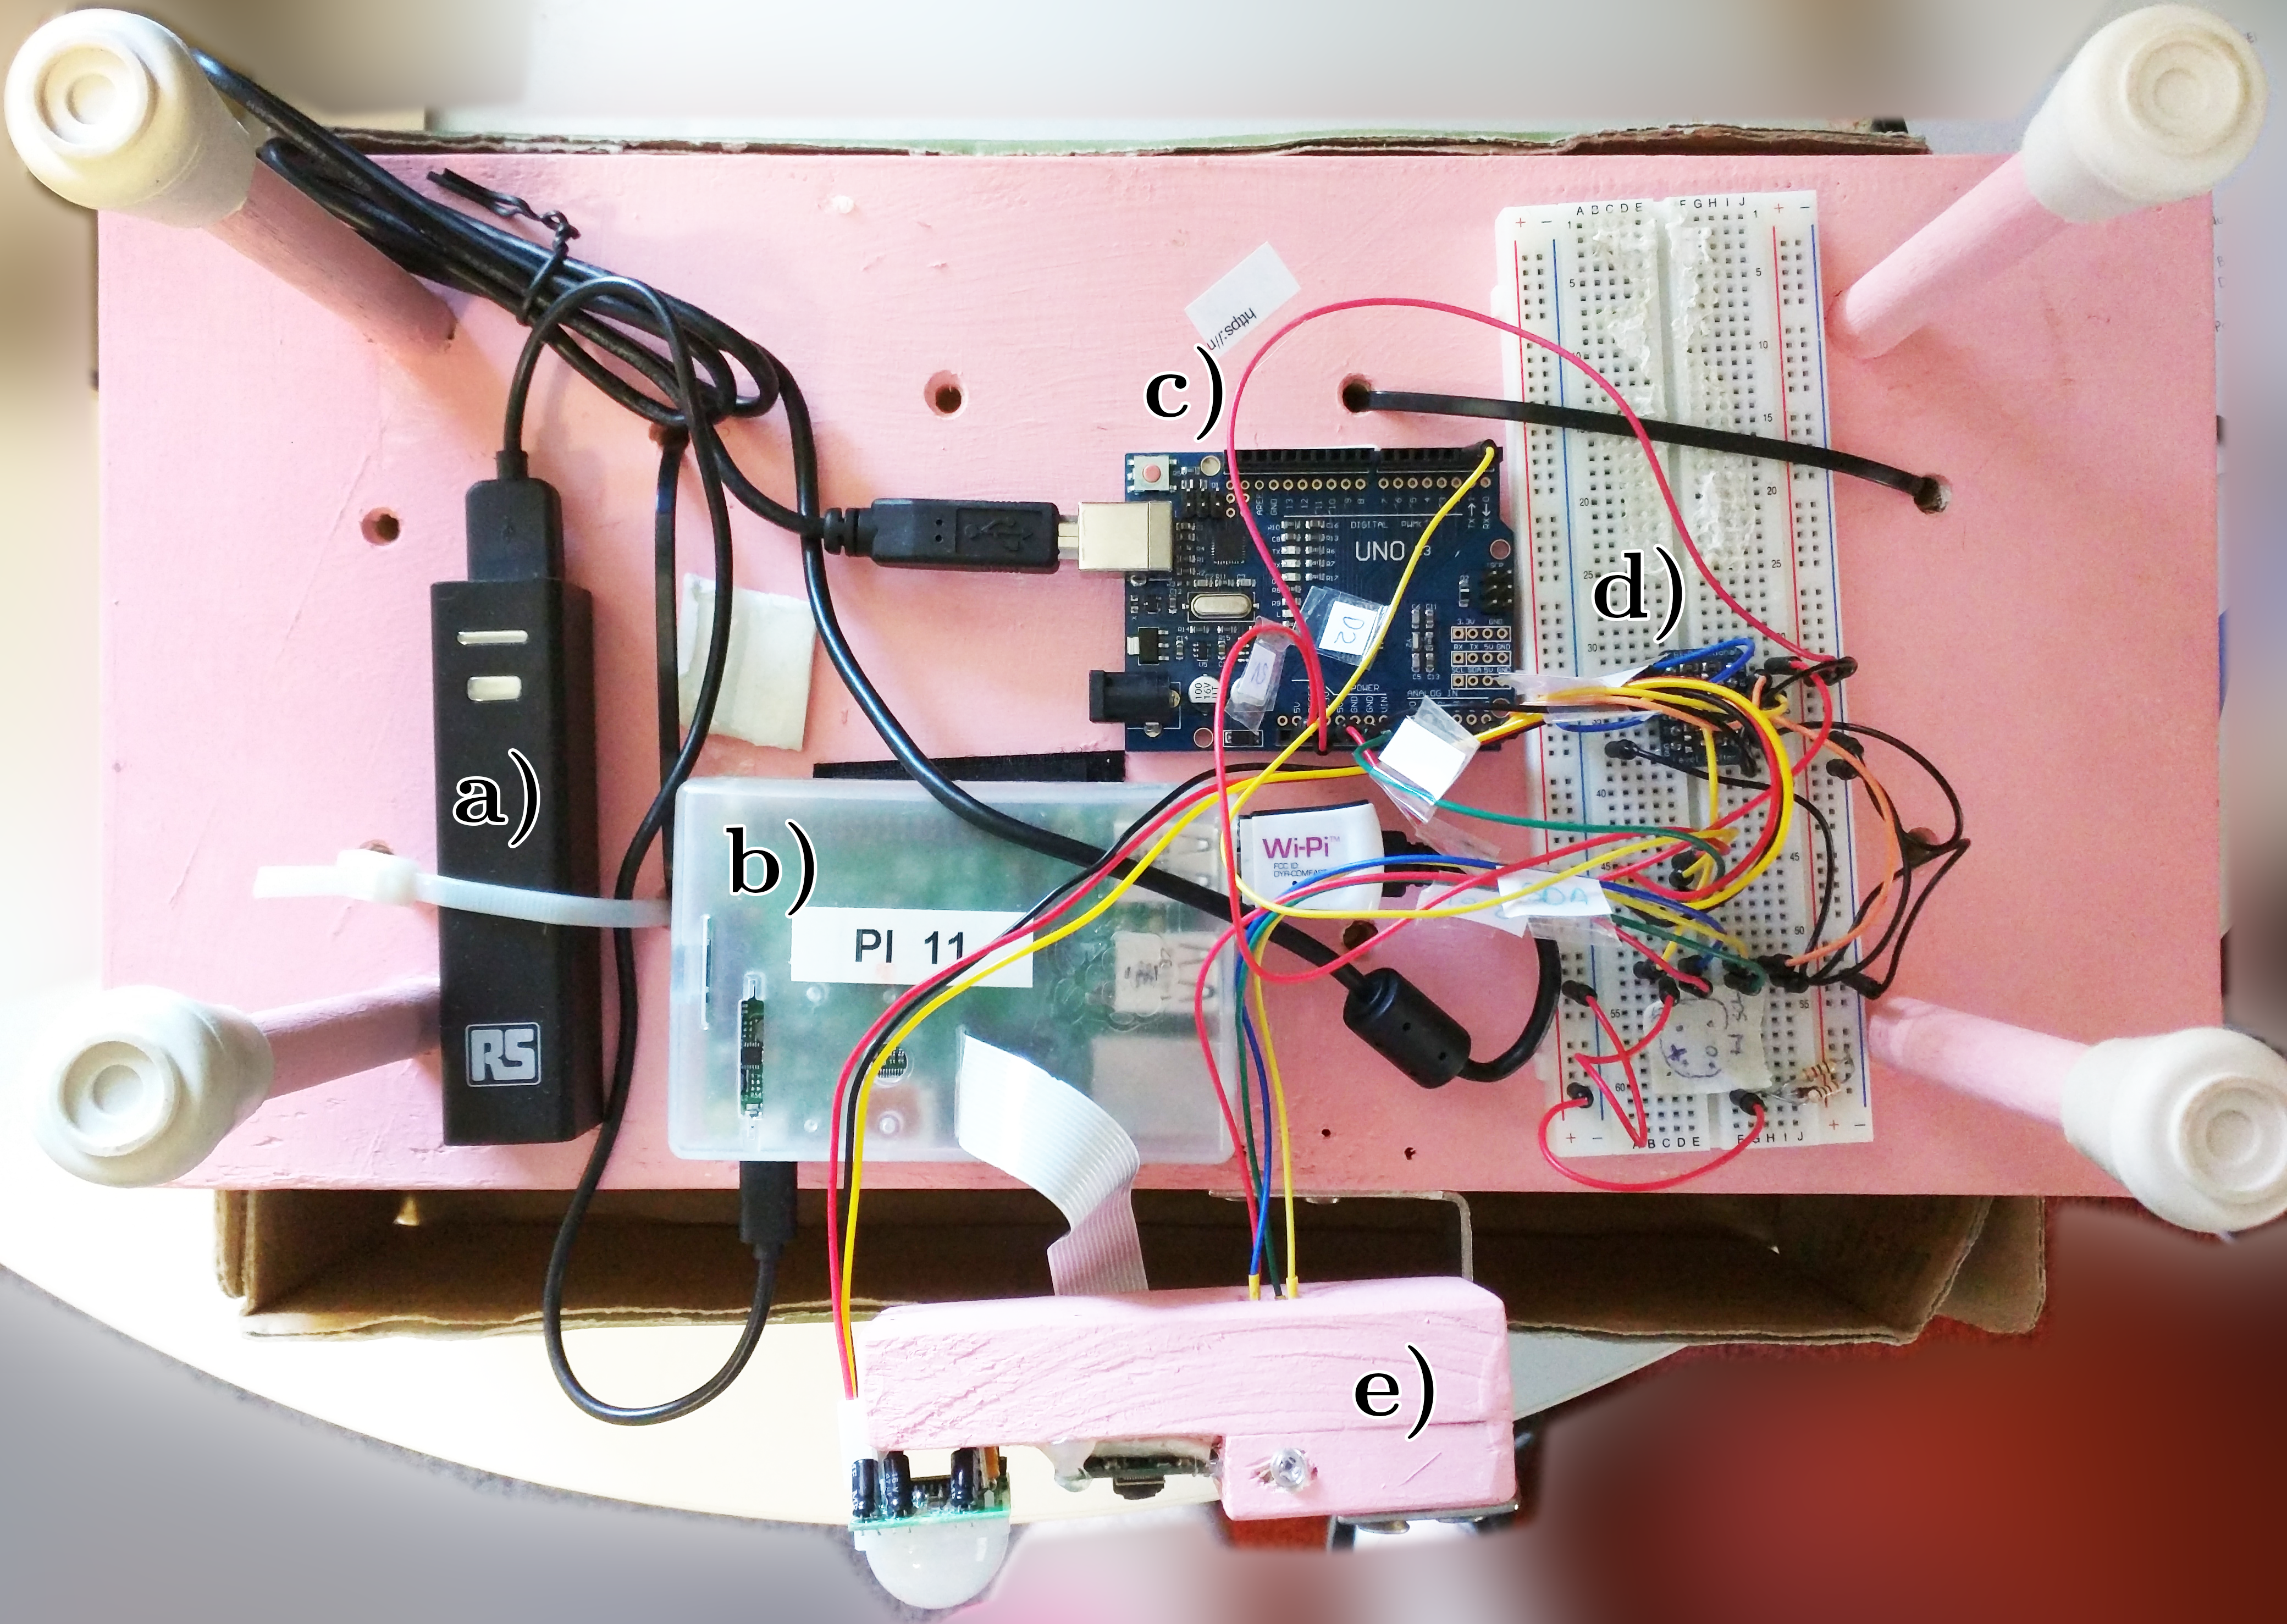
\includegraphics[width=\textwidth]{../diagrams/prototypeb-1.jpg}
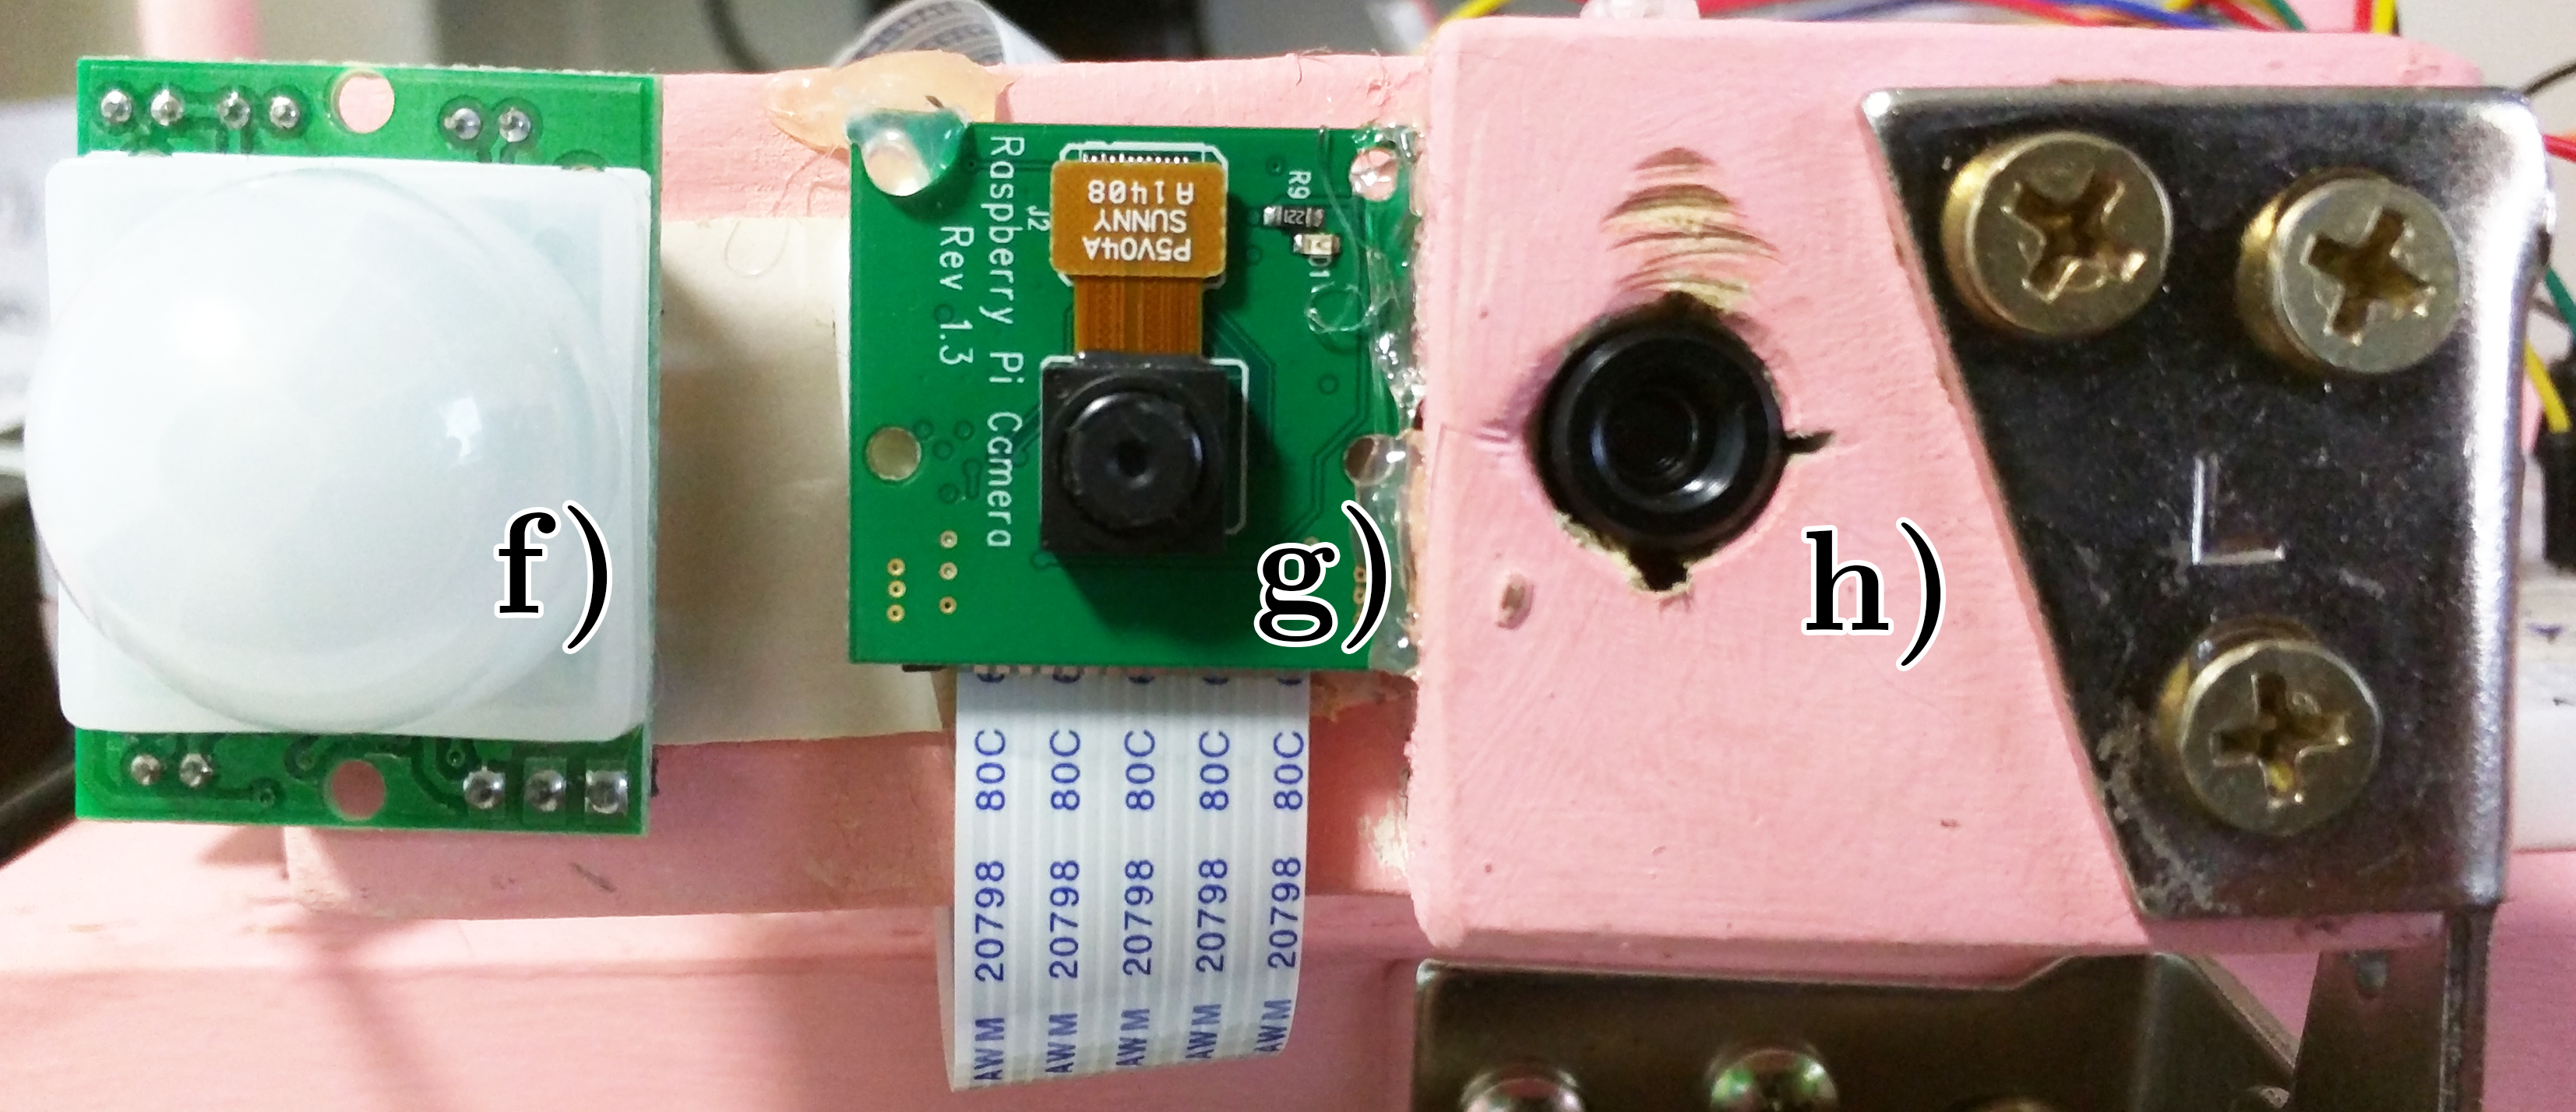
\includegraphics[width=\textwidth]{../diagrams/prototypeb-2.jpg}
{\small
\begin{multicols}{2}
\begin{enumerate}[a)]
 \item Battery pack
 \item Raspberry Pi
 \item Arduino
 \item Level-shifting circuitry
 \item Movable sensor mount
 \item PIR
 \item Camera
 \item \mlx
\end{enumerate}
\end{multicols}
}
\caption{Prototype Physical Form}
\label{fig:pictures:protob1}
\end{figure}

\chapter{Original Honours Proposal}
\subfile{../proposal/proposal}
%TC:endignore

\end{document}